\documentclass[a4paper]{article}
\usepackage[italian]{babel}
\usepackage[T1]{fontenc}
\usepackage[utf8]{inputenc}
\usepackage{graphicx}
\usepackage[margin=1in]{geometry}
\usepackage{makecell}
%\usepackage[svgnames,table]{xcolor}
\usepackage[table]{xcolor}
% --- Per lo sfondo
%\usepackage{eso-pic,graphicx}
% ---
\usepackage{setspace}

\usepackage{tabularx} 

\usepackage{hyperref}
\usepackage{array}

\usepackage{fancyhdr}

% Definizione comandi personali - Team
\newcommand{\FP}{Francesco Protopapa}
\newcommand{\GC}{Greta Cavedon}
\newcommand{\LW}{Luciano Wu}
\newcommand{\PV}{Pietro Villatora}
\newcommand{\EP}{Edoardo Pavan}
\newcommand{\MG}{Michele Gatto}
\newcommand{\MB}{Matteo Basso}

% Definizione File
\newcommand{\G}{\textit{Glossario v1.0.0}}
\newcommand{\AdR}{\textit{Analisi dei Requisiti v1.0.0}}
\newcommand{\PdP}{\textit{Piano di Progetto v1.0.0}}
\newcommand{\PdQ}{\textit{Piano di Qualifica v1.0.0}}
\newcommand{\SdF}{\textit{Studio di fattibilità v1.0.0}}
\newcommand{\NdP}{\textit{Norme di Progetto v1.0.0}}

% Definizione ruoli
\newcommand{\AN}{Analista}
\newcommand{\VE}{Verificatore}
\newcommand{\AM}{Amministratore}
\newcommand{\RE}{Responsabile}
\newcommand{\PT}{Progettista}
\newcommand{\PR}{Programmatore}

\newcommand{\glo}{\textsuperscript{G}}

%Abbreviaizoni requisiti
\newcommand{\Ob}{Obbligatorio}
\newcommand{\De}{Desiderabile}
\newcommand{\Fa}{Facoltativo}

%Abbrevizioni fonti requisiti
\newcommand{\Di}{Decisione interna}
\newcommand{\Vi}{Verbale interno}
\newcommand{\Ve}{Verbale esterno}
\newcommand{\Ca}{Capitolato}

%link in blu
\newcommand{\mylink}[1]{\color{blue}\url{#1}\color{black}}
\makeindex

\usepackage{hyperref}

\usepackage{longtable}

% Per evidenziare il testo
\usepackage{tcolorbox}




\begin{document}

	% Intro documento 

\begin{center}

\begin{figure}
\centering

\includegraphics[scale=0.05]{Contenuto/Immagini/DreamTeam.png} 
\end{figure}

{\Huge{\textbf{Norme di Progetto}}} \\ [1cm]

\begin{table}[htbp]
\centering
\begin{tabular}{r|c}
\multicolumn{2}{c}{\textbf{Informazioni sul Documento}} \\
\hline \\
\textbf{Versione} & 3.0.0 \\ \rule{0pt}{3ex}    
\textbf{Data di approvazione} & 2022-06-18  \\ \rule{0pt}{2ex} 
\textbf{Approvatori} & \MB{} \\ \rule{0pt}{3ex}      
\textbf{Redattori} & \MG{} \\ \rule{0pt}{2ex}   
& \PV{} \\ \rule{0pt}{3ex}    
\textbf{Verificatori} 
  & \GC{} \\ \rule{0pt}{2ex}
& \EP{} \\ \rule{0pt}{2ex} 
      
\textbf{Uso} & Interno \\ \rule{0pt}{3ex}    
\textbf{Distribuzione} & Prof. Vardanega Tullio \\ \rule{0pt}{2ex}   
& Prof. Cardin Riccardo \\ \rule{0pt}{2ex}   
& Gruppo \textit{DreamTeam} \\ \rule{0pt}{0.1cm}   
\end{tabular} \\ [0.5cm]
\end{table}

\textsl{ e-mail: \href{mailto:dreamteam.unipd@gmail.com}{dreamteam.unipd@gmail.com} } \\[2cm]
\end{center}
\pagebreak	
	% Inserimento di header e footer

\pagestyle{fancy}
\fancyhf{}
\rhead{Analisi dei Requisiti}
\lhead{
\includegraphics[scale=0.015]{Sezioni/images/DreamTeam.png}}
\rfoot{\thepage}
\setlength{\headheight}{35pt}

%\cfoot{Pagina \thepage}
%\setlength{\headheight}{35pt}
%\setcounter{tocdepth}{5}
%\setcounter{secnumdepth}{5}
%\renewcommand{\footrulewidth}{0.4pt}
	% Registro Modifiche

{\LARGE{\textbf{Registro delle Modifiche}}} \\
\begin{table}[!htbp]
\begin{tabular}{|m{0.1\textwidth}<{\centering}|m{0.1\textwidth}<{\centering}|m{0.2\textwidth}<{\centering}|m{0.2\textwidth}<{\centering}|m{0.3\textwidth}<{\centering}|}
	\hline \rowcolor{gray!50}
	\textbf{Versione}&\textbf{Data}&\textbf{Nominativo}&\textbf{Ruolo}&\textbf{Descrizione}\\ 
	\hline
	0.1.0& 06.12.21& \shortstack{ } &\shortstack{ \\ \VE{} } & Verifica del corretto output del documento in latex\\
	\hline
	0.0.3& 06.12.21& \shortstack{ \\ \GC{}} &\shortstack{ \\ \AN{} } & Conversione del documento in latex\\
	\hline
	0.0.2& 01.12.21& \shortstack{ \\ \FP{},\\ \LW{}} &\shortstack{ \\ \AN{}, \\ \AN{}} & Inserimento altri termini e relativi significati\\
	\hline
	0.0.1& 29.11.21& \shortstack{ \\ \GC{}} &\shortstack{ \\ \AN{} } & Creazione bozza del documento, ricerca dei primi termini e relativi significati\\
	\hline
\end{tabular}
\end{table}

\pagebreak	

	% indice
	\renewcommand{\contentsname}{Indice}
	\tableofcontents	
	\pagebreak
	
	% contenuto del documento, ogni sezione in un file
	\section{Introduzione}

\subsection{Scopo del Documento}
Lo scopo di questo documento è di descrivere dettagliatamente i requisiti del progetto definendone i casi d’uso individuati nello studio del progetto.

\subsection{Scopo del Prodotto}

L’obiettivo di Sweeat e dell’azienda Zero12 è la creazione di un sistema software costituito da una Webapp. Lo scopo del prodotto è di fornire all’utente una guida dei locali gastronomici sfruttando i numerosi contenuti digitali creati dagli utenti sulle principali piattaforme social (Instagram e TikTok). In questo modo, è possibile realizzare una classifica basata sulle impressioni e reazioni di chiunque usufruisca dei servizi dei locali, non solo da professionisti ed esperti del settore.

\subsection{Glossario}

Per evitare ambiguità relative alle terminologie utilizzate è stato creato un documento denominato “\textit{Glossario}”. Questo documento comprende tutti i termini tecnici scelti dai membri del gruppo e utilizzati nei vari documenti con le relative definizioni. Tutti i termini inclusi in questo glossario, vengono segnalati all’interno del documento con l’apice\textsuperscript{G} accanto alla parola.

\subsection{Riferimenti}

\subsubsection{Riferimenti normativi}
\begin{itemize}
    \item \NdP{};
    \item Verbale Esterno 2021-12-22;
    \item Presentazione del capitolato - Zero12 Progettazione e sviluppo di una Social guida Michelin: \newline \mylink{https://www.math.unipd.it/~tullio/IS-1/2021/Progetto/C4p.pdf}.
\end{itemize}
\subsubsection{Riferimenti informativi}
\begin{itemize}
    \item Casi d'uso - Materiale didattico del corso di Ingegneria del Software: \newline\mylink{https://www.math.unipd.it/~rcardin/swea/2022/Diagrammi\%20Use\%20Case.pdf};
    \item Analisi dei requisiti - Materiale didattico del corso di Ingegneria del Software: \newline \mylink{ https://www.math.unipd.it/~tullio/IS-1/2021/Dispense/T07.pdf};
    \item Regolamento del progetto didattico - Materiale didattico del corso di Ingegneria del Software:\newline \mylink{https://www.math.unipd.it/~tullio/IS-1/2021/Dispense/PD2.pdf}.
\end{itemize}


 	
	\pagebreak %si possono eventualmente togliere per accorciare lo spazio
	\section{Descrizione Generale}

\subsection{Caratteristiche del Prodotto}

A seguito della presentazione del capitolato\textsuperscript{G} e dei primi incontri fatti con il proponente\textsuperscript{G} è emerso che il prodotto che andremo a realizzare dovrà avere le seguenti caratteristiche:

\subsubsection{Crawling dei dati da Instagram e TikTok}
Il team dovrà effettuare un’analisi mediante le API\textsuperscript{G} social di Instagram e TikTok per capire se esse sono sufficienti a raccogliere e analizzare le informazioni, in caso contrario si dovrà individuare una soluzione alternativa per effettuare tali operazioni. In ogni caso si dovranno analizzare esclusivamente profili pubblici ed escogitare una strategia per evitare di essere inseriti nelle black-list\textsuperscript{G} di Instagram e TikTok a causa di queste operazioni.

\subsubsection{Traduzione dei dati ottenuti}
Nella fase di crawling verranno raccolti dati di diverso tipo quali foto, video, stories, post e commenti. Questi dati andranno poi “tradotti” utilizzando diversi servizi come ad esempio Amazon Rekognition\textsuperscript{G} e Amazon Comprehend\textsuperscript{G} in modo da assegnare a ciascun dato un valore quantitativo relativo alla sua positività. Bisognerà inoltre riconoscere tutti i dati raccolti che non sono assolutamente rilevanti, i quali verranno scartati. Particolare attenzione andrà prestata ai commenti, riguardo i quali è richiesto di svolgere un’analisi preliminare al fine di capire se è davvero utile includerli nella raccolta dei dati.

\subsubsection{Realizzazione di un ranking}
Sarà compito del team progettare un sistema di ranking\textsuperscript{G} dei locali presenti nella guida, in particolare bisognerà decidere che peso dare a ciascun tipo di contenuto e fare attenzione a considerare anche dati che apparentemente non sembrano significativi ma che correlati con altri possono assumere un significato ben preciso, come ad esempio due foto postate in successione dallo stesso profilo\textsuperscript{G} in cui nella prima si vede un ristorante e nella seconda una persona felice. Sarà inoltre necessario decidere in base a che criteri strutturare il ranking, i quali potrebbero essere la regione in cui si trova il locale, il tipo di cucina o altri. Per questa fase non sono state stabilite delle linee guida molto rigide e viene lasciata molta libertà al team per l’implementazione.

\subsubsection{Interfaccia utente}
L’utente\textsuperscript{G} potrà interfacciarsi con la guida tramite una WebApp\textsuperscript{G} la quale dovrà fornire alcune funzionalità principali quali la visualizzazione del ranking, la ricerca di uno specifico locale per la consultazione delle informazioni principali e del suo punteggio, la possibilità di registrarsi e poter suggerire nuovi profili\textsuperscript{G} social da cui andare a effettuare il crawling dei dati.

\subsection{Caratteristiche degli Utenti}

La piattaforma\textsuperscript{G} offre la possibilità di poter consultare la guida tramite WebApp sia ad utenti non autenticati che ad utenti autenticati\textsuperscript{G}. Ciascuna tipologia di utente potrà avere accesso a funzionalità differenti.

\subsubsection{Utente Non Autenticato}

Con il termine utente non autenticato\textsuperscript{G} ci si riferisce ad una qualsiasi persona non autenticata nel sistema, che può sfruttare le funzionalità di base offerte dalla piattaforma, ossia:

\begin{itemize}
  \item Visualizzare il ranking dei locali\textsuperscript{G} applicando specifici filtri\textsuperscript{G};
  \item Cercare un determinato locale attraverso la funzionalità di ricerca;
  \item Consultare il profilo social di un locale, conoscerne gli orari di apertura ed il numero di telefono, oltre a visitare il sito web (nel caso esista);
  \item Registrarsi nella piattaforma per sfruttare delle funzionalità aggiuntive.
\end{itemize}

\subsubsection{Utente Autenticato}

Invece, con il termine “utente autenticato” ci si riferisce ad una persona registrata nel database e che ha effettuato l'accesso nella piattaforma, la quale, oltre a sfruttare le funzionalità dell’utente generico\textsuperscript{G}, può anche:

\begin{itemize}
  \item Suggerire nuovi profili dai quali andare ad effettuare il crawling dei dati per realizzare il \textsuperscript{G};
  \item Creare liste personalizzate private\textsuperscript{G} con i locali preferiti\textsuperscript{G};
  \item Gestire il profilo personale (modificare la password, collegare l'account Instagram e/o TikTok).
\end{itemize}

% \subsubsection{WebApp}

% Tra le caratteristiche del prodotto, troviamo anche la realizzazione di una WebApp che permetterà all'utente finale di poter fruire dei contenuti presenti nella piattaforma.

% Una WebApp\textsuperscript{G}{} è un'applicazione formata da più pagine web accessibili tramite un browser (ad esempio: Google Chrome, Firefox, Safari, Microsoft Edge ed Opera). Al fine di ottenere la miglior esperienza utente possibile, è consigliabile consultare la piattaforma usando un browser (tra quelli appena elencati) nella sua versione più aggiornata.

\subsection{Obblighi di Progettazione}

\begin{itemize}
  \item Creare e sfruttare delle API\textsuperscript{G} per il crawling\textsuperscript{G} dei dati se quelle già esistenti non sono sufficienti allo scopo del prodotto;
  \item Valutare strategie Voice to Text se le informazioni quali testi, commenti e tag non sono sufficienti;
  \item Realizzare una WebApp\textsuperscript{G} con design responsive per permettere agli utenti di consultare i contenuti presenti nella piattaforma ed usufruire di tutte le sue funzionalità;
  \item Utilizzo di un'architettura a microservizi\textsuperscript{G}{}.
\end{itemize}

\subsubsection{Tecnologie utilizzate}

Per sviluppare la piattaforma verranno utilizzare le seguenti tecnologie:
\begin{itemize}
    \item \textbf{Python\textsuperscript{G}} per la creazione e l'utilizzo dai crawler\textsuperscript{G} che estrapolerà i dati dai contenuti social;
    \item \textbf{HTML5\textsuperscript{G}}: per creare la struttura dell'interfaccia utente;
    \item \textbf{CSS3\textsuperscript{G}}: per lo stile dell'interfaccia utente;
    \item \textbf{React\textsuperscript{G}} per la creazione dell'interfaccia\textsuperscript{G} utente;
    \item \textbf{AWS\textsuperscript{G}} tramite i seguenti servizi:
    \begin{itemize}
    	\item \textbf{Amazon Rekognition} per analizzare e riconoscere attributi\textsuperscript{G}{}, oggetti e testi dei contenuti multimediali;
    	\item \textbf{Amazon Comprehend} per analizzare e riconoscere informazioni presenti nei contenuti testuali;
    	\item \textbf{AWS Lambda\textsuperscript{G}} per il crawler, l'inserimento e l'estrazione dei dati nel/dal database;
    	\item \textbf{Amazon Aurora Serverless\textsuperscript{G}} con \textbf{MySQL} come database relazionale;
    	\item \textbf{Amazon S3\textsuperscript{G}} per l'archiviazione di documenti;
    	\item \textbf{API Gateway\textsuperscript{G}} per consentire alla WebApp di visualizzare i contenuti;
    	\item \textbf{Amazon Amplify\textsuperscript{G}} che consiste in un set di strumenti che permettono di realizzare e far funzionare correttamente la WebApp.
	\end{itemize}
  \end{itemize} 	
	\pagebreak
	
	%\section{Casi D'Uso}
%\subsection{Introduzione}
In questa sezione verranno presentati i casi d’uso individuati dal gruppo DreamTeam, i quali fanno riferimento a tutte le funzionalità che la piattaforma Sweeat dovrà offrire ad ogni utente che vorrà interfacciarsi con essa.
\subsection{Attori primari}
\begin{itemize}
    \item \textbf{Utente non Autenticato}: utente che non ha ancora effettuato la fase di autenticazione sulla piattaforma. Può essere in possesso o meno delle credenziali per l’autenticazione. Avrà funzionalità limitate rispetto ad un utente autenticato;
    \item \textbf{Utente Autenticato}: utente che ha effettuato l’autenticazione alla piattaforma tramite le proprie credenziali. Ha accesso ad ogni funzionalità messa a disposizione dalla piattaforma;
    \item \textbf{Utente Generico}: può essere sia un utente autenticato che un utente non autenticato.
\end{itemize}
\subsection{Attori secondari}
\begin{itemize}
    \item \textbf{Instagram}: servizio di rete sociale statunitense che permette agli utenti di scattare foto, applicarvi filtri e condividerle via Internet;
    \item \textbf{TikTok}: social network cinese attraverso cui gli utenti possono creare brevi clip musicali.
\end{itemize}
\clearpage 
	\subsection{UC1 - Utente Non Autenticato}

\subsubsection{UC1.1 - Registrazione}
\begin{center}
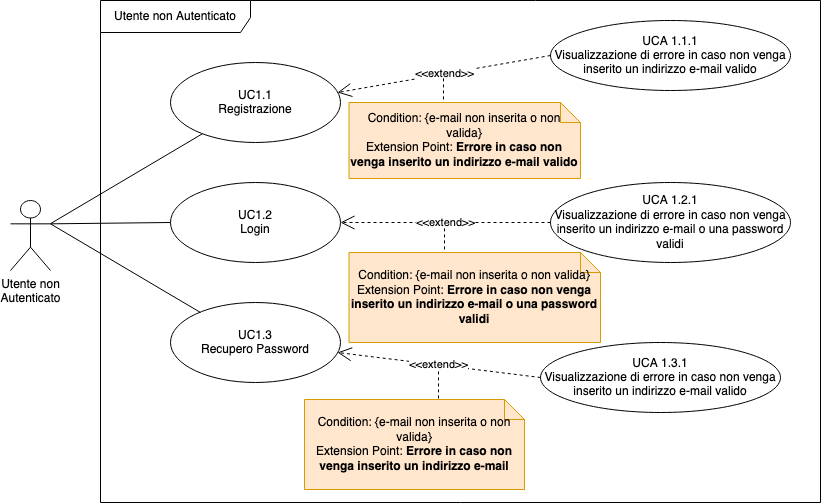
\includegraphics[scale=0.5]{UC_images/UC1.png}
\end{center}
\begin{itemize}
\item \textbf{Attore primario}: Utente non autenticato.
\item \textbf{Precondizione}: L'utente non è ancora autenticato presso il sistema.
\item \textbf{Postcondizione}: L’utente possiede un account con cui può accedere al sistema, contraddistinto da una username ed una password.

\item \textbf{Scenario principale}:
\begin{enumerate}
\item L’utente accede al sistema;
\item L’utente seleziona la funzionalità “Registrati”;
\item L'utente inserisce i campi dati obbligatori: Nome e Cognome;
\item L’utente inserisce un indirizzo e-mail univoco nel campo username non ancora utilizzato con cui accedere al sistema; 
\item L’utente inserisce una password per accedere al sistema;
\item Affinché la registrazione vada a buon fine, l’utente dovrà cliccare su “Registrati”.
\end{enumerate}

\item \textbf{Estensioni}:
\begin{itemize}
\item Nel caso in cui l’utente inserisca un indirizzo e-mail non esistente, già presente a sistema o lasci il campo vuoto
\begin{enumerate}
	\item L’utente non viene registrato nel sistema;
	\item Viene mostrato un messaggio d’errore che indica che l'indirizzo e-mail inserito non è corretto (UC1.1.1 §).
\end{enumerate}
\item Nel caso in cui l’utente provi a registrarsi inserendo una password più breve di 8 caratteri
\begin{enumerate}
	\item L’utente non viene registrato nel sistema;
	\item Viene mostrato un messaggio d’errore che indica che non è stata inserita alcuna password (UC1.1.2 §).
\end{enumerate}
\item{Nel caso in cui l'utente non inserisca il proprio nome e cognome}
\begin{enumerate}
	\item L'utente non viene registrato nel sistema;
	\item Viene mostrato un messaggio d'errore che indica che il nome ed il cognome non sono stati inseriti correttamente (UC1.1.3 §).
\end{enumerate}
\end{itemize}
\end{itemize}

\subsubsection{UC1.1.1 - Errore inserimento e-mail}
\begin{itemize}
\item \textbf{Attore primario}: Utente non autenticato.
\item \textbf{Precondizione}: L'utente non è ancora autenticato presso il sistema.
\item \textbf{Postcondizione}: Viene mostrato un messaggio d'errore e l'utente non viene autenticato nel sistema.

\item \textbf{Scenario principale}:
\begin{enumerate}
\item L'operazione di inserimento dell'indirizzo e-mail fallisce;
\item Viene mostrato il corrispondente messaggio d'errore;
\item All'utente viene data la possibilità di tentare nuovamente la registrazione al sistema.
\end{enumerate}
\end{itemize}

\subsubsection{UC1.1.2 - Errore inserimento password}
\begin{itemize}
\item \textbf{Attore primario}: Utente non autenticato.
\item \textbf{Precondizione}: L'utente non è ancora autenticato presso il sistema.
\item \textbf{Postcondizione}: Viene mostrato un messaggio d'errore e l'utente non viene autenticato nel sistema.

\item \textbf{Scenario principale}:
\begin{enumerate}
\item L'operazione di inserimento password fallisce;
\item Viene mostrato il corrispondente messaggio d'errore;
\item All'utente viene data la possibilità di tentare nuovamente la registrazione al sistema.
\end{enumerate}
\end{itemize}

\subsubsection{UC1.1.3 - Errore inserimento dati personali}
\begin{itemize}
\item \textbf{Attore primario}: Utente non autenticato.
\item \textbf{Precondizione}: L'utente non è ancora autenticato presso il sistema.
\item \textbf{Postcondizione}: Viene mostrato un messaggio d'errore e l'utente non viene autenticato nel sistema.

\item \textbf{Scenario principale}:
\begin{enumerate}
\item L'operazione di inserimento dei dati personali (Nome e Cognome) fallisce;
\item Viene mostrato il corrispondente messaggio d'errore;
\item All'utente viene data la possibilità di tentare nuovamente la registrazione al sistema.
\end{enumerate}
\end{itemize}

\subsubsection{UC1.2 - Login}
\begin{itemize}
\item \textbf{Attore primario}: Utente non autenticato.
\item \textbf{Precondizione}: L'utente non è ancora autenticato presso il sistema.
\item \textbf{Postcondizione}: L’utente ha effettuato l’accesso al sistema ed è all’interno del proprio account.

\item \textbf{Scenario principale}:
\begin{enumerate}
\item L’utente accede al sistema;
\item L’utente seleziona la voce “Login”;
\item L’utente inserisce l’indirizzo e-mail con cui è registrato al sistema;
\item L’utente inserisce la password d’accesso; 
\item L’utente seleziona la voce “Login”. 
\end{enumerate}

\item \textbf{Estensioni}:
\begin{itemize}
\item Viene inserito uno username errato / non registrato
\begin{enumerate}
	\item L’utente non può accedere al sistema;
	\item Viene mostrato un messaggio d’errore che indica che lo username inserito non è corretto (UC1.2.1 §). 
\end{enumerate}
\item Viene inserita una password errata
\begin{enumerate}
	\item L’utente non può accedere al sistema;
	\item Viene mostrato un messaggio d’errore che indica che la password inserita non è corretta (UC1.2.2 §).
\end{enumerate}
\end{itemize}
\end{itemize}

\subsubsection{UC1.2.1 - Errore inserimento username}
\begin{itemize}
\item \textbf{Attore primario}: Utente non autenticato.
\item \textbf{Precondizione}: L'utente non è ancora autenticato presso il sistema.
\item \textbf{Postcondizione}: Viene mostrato un messaggio d'errore e l'utente non viene autenticato nel sistema.

\item \textbf{Scenario principale}:
\begin{enumerate}
\item L'operazione di inserimento dello username fallisce;
\item Viene mostrato il corrispondente messaggio d'errore;
\item All'utente viene data la possibilità di tentare nuovamente l'accesso al sistema.
\end{enumerate}
\end{itemize}

\subsubsection{UC1.2.2 - Errore inserimento password}
\begin{itemize}
\item \textbf{Attore primario}: Utente non autenticato.
\item \textbf{Precondizione}: L'utente non è ancora autenticato presso il sistema.
\item \textbf{Postcondizione}: Viene mostrato un messaggio d'errore e l'utente non viene autenticato nel sistema.

\item \textbf{Scenario principale}:
\begin{enumerate}
\item L'operazione di inserimento dello username fallisce;
\item Viene mostrato il corrispondente messaggio d'errore;
\item All'utente viene data la possibilità di tentare nuovamente l'accesso al sistema.
\end{enumerate}
\end{itemize}

\subsubsection{UC1.3 - Password Dimenticata}
\begin{itemize}
\item \textbf{Attore primario}: Utente non autenticato.
\item \textbf{Precondizione}: L’utente non è ancora autenticato presso il sistema.
\item \textbf{Postcondizione}: L’utente ha la possibilità di recuperare la password tramite l'indirizzo e-mail con cui è registrato nella piattaforma.

\item \textbf{Scenario principale}:
\begin{enumerate}
\item L’utente accede al sistema;
\item L’utente seleziona la voce “Login”;
\item L’utente clicca sulla voce “Password dimenticata”;
\item L’utente inserisce l’indirizzo e-mail da cui recuperare la password;
\item L’utente clicca su “Recupera password”. 
\end{enumerate}

\item \textbf{Estensioni}:
\begin{itemize}
\item Viene inserito un indirizzo e-mail non valido / non registrato
\begin{enumerate}
	\item L’utente non può recuperare la password;
	\item Viene mostrato un messaggio d’errore che indica che l’indirizzo e-mail inserito non è corretto (UC1.2.2 §).
\end{enumerate}
\end{itemize}
\end{itemize}


	\subsection{UC2 - Area Personale}
\begin{center}
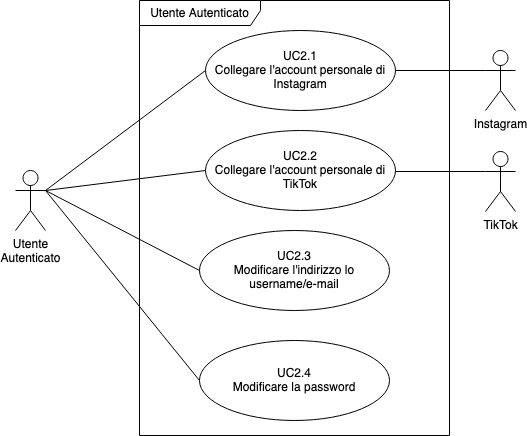
\includegraphics[scale=0.5]{UC_images/UC2.png}
\end{center}
\subsubsection{UC2.1 - Collegare l'Account Instagram}
\begin{center}
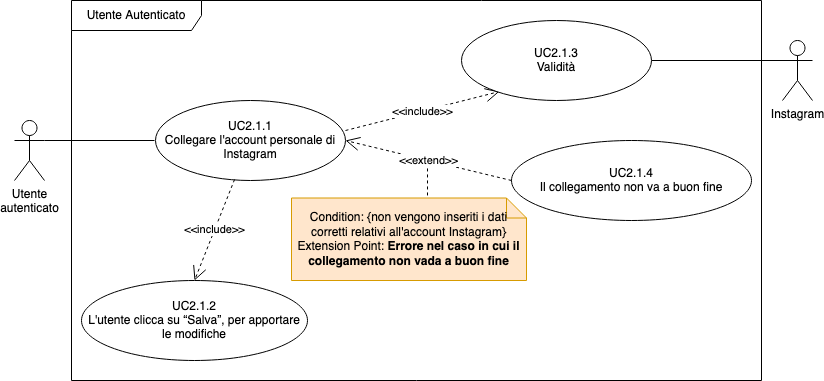
\includegraphics[scale=0.5]{UC_images/UC2_1.png}
\end{center}
\begin{itemize}
\item \textbf{Attore primario}: Utente autenticato
\item \textbf{Attore secondario}: Instagram
\item \textbf{Precondizione}: L’utente è autenticato nel sistema
\item \textbf{Postcondizione}: L’utente ha collegato il suo account Instagram al sistema

\item \textbf{Scenario principale}:
\begin{enumerate}
\item L’utente collega il suo account personale di Instagram
\item Per confermare l’azione, l’utente deve cliccare su “Salva” 
\end{enumerate}

\item \textbf{Estensioni}:
\begin{itemize}
\item Il collegamento all’account Instagram non va a buon fine
\begin{enumerate}
	\item L’utente prova a collegare il proprio account Instagram all’account registrato nel sistema, cliccando il bottone “Instagram”;
	\item L’accesso alla piattaforma Instagram non va a buon fine, poiché non vengono inseriti i dati di accesso corretti (UC2.1.4 §).
	%\item All’utente viene offerta la possibilità di effettuare un nuovo collegamento
\end{enumerate}
\end{itemize}

\item \textbf{Inclusioni}:
\begin{itemize}
\item Verifica validità link (UC3.2 §3.8).
\end{itemize}
\end{itemize}

\subsubsection{UC2.2 - Collegare l'Account TikTok}
\begin{center}
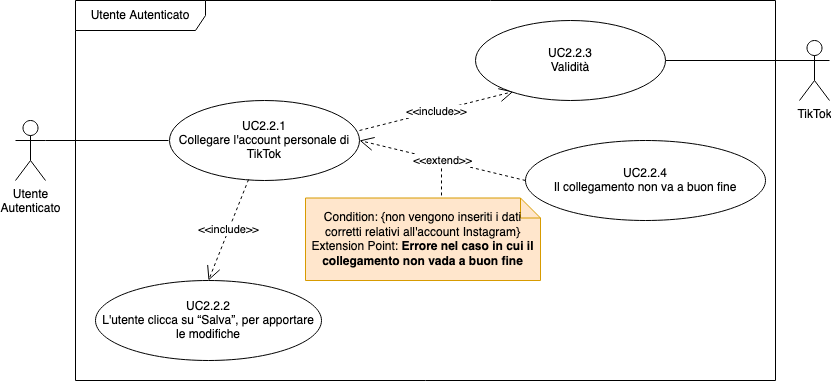
\includegraphics[scale=0.5]{UC_images/UC2_2.png}
\end{center}
\begin{itemize}
\item \textbf{Attore primario}: Utente autenticato.
\item \textbf{Attore secondario}: TikTok.
\item \textbf{Precondizione}: L’utente è autenticato nel sistema.
\item \textbf{Postcondizione}: L’utente ha collegato il suo account TikTok al sistema.

\item \textbf{Scenario principale}:
\begin{enumerate}
\item L’utente collega il suo account personale di TikTok;
\item Per confermare l’azione, l’utente deve cliccare su “Salva”. 
\end{enumerate}

\item \textbf{Estensioni}:
\begin{itemize}
\item Il collegamento all’account Instagram non va a buon fine
\begin{enumerate}
	\item L’utente prova a collegare il proprio account TikTok all’account registrato nel sistema, cliccando il bottone TikTok;
	\item L’accesso alla piattaforma TikTok non va a buon fine, poiché non vengono inseriti i dati di accesso corretti (UC2.2.4 §).
\end{enumerate}
\end{itemize}

\item \textbf{Inclusioni}:
\begin{itemize}
\item Verifica validità link (UC3.2 §3.8).
\end{itemize}
\end{itemize}

\subsubsection{UC2.3 - Modifica dell'indirizzo e-mail/username}
\begin{center}
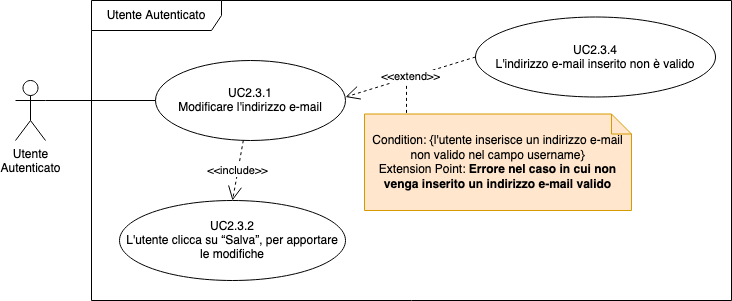
\includegraphics[scale=0.5]{UC_images/UC2_3.png}
\end{center}
\begin{itemize}
\item \textbf{Attore primario}: Utente autenticato.
\item \textbf{Precondizione}: L’utente è autenticato nel sistema.
\item \textbf{Postcondizione}: L’utente ha inserito un indirizzo e-mail valido ed ha modificato il campo e-mail/username.

\item \textbf{Scenario principale}:
\begin{enumerate}
\item L’utente inserisce il nuovo indirizzo e-mail nel campo e-mail/username;
\item L’utente clicca su “Salva” per aggiornare l'indirizzo e-mail registrato nella piattaforma.
\end{enumerate}

\item \textbf{Estensioni}:
\begin{itemize}
\item L’utente inserisce un indirizzo e-mail non valido
\begin{enumerate}
	\item L’utente inserisce un nuovo indirizzo e-mail nel campo e-mail/username;
	\item Il sistema rileva che l’indirizzo inserito non è valido (UC2.3.4 §).
	%\item Il sistema non modifica l’indirizzo e-mail e mantiene il vecchio indirizzo;
	%\item All’utente viene data la possibilità di modificare lo username inserendo nuovamente un indirizzo e-mail valido.
\end{enumerate}
\end{itemize}
\end{itemize}

\subsubsection{UC2.4 - Modifica della password}
\begin{center}
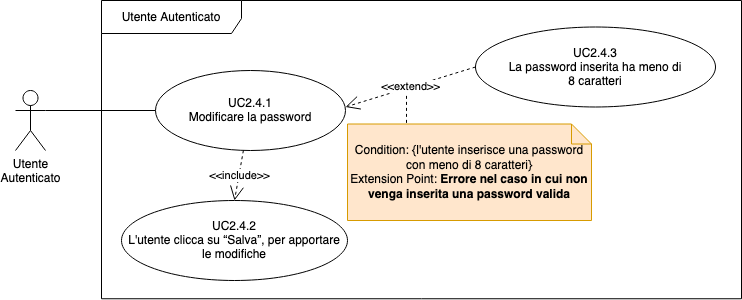
\includegraphics[scale=0.5]{UC_images/UC2_4.png}
\end{center}
\begin{itemize}
\item \textbf{Attore primario}: Utente autenticato
\item \textbf{Precondizione}: L’utente è autenticato nel sistema
\item \textbf{Postcondizione}: L’utente ha modificato con successo la password per l’accesso al sistema

\item \textbf{Scenario principale}:
\begin{enumerate}
\item L’utente digita la nuova password nel campo password;
\item L’utente clicca su “Salva” per aggiornare la password con cui accedere al sistema.
\end{enumerate}

\item \textbf{Estensioni}:
\begin{itemize}
\item Viene inserita una password con meno di 8 caratteri
\begin{enumerate}
	\item L'utente inserisce una password non valida (UC2.4.3 §).
\end{enumerate}
\end{itemize}
\end{itemize}
	\subsection{UC3 – Proposta profilo}
\begin{center}
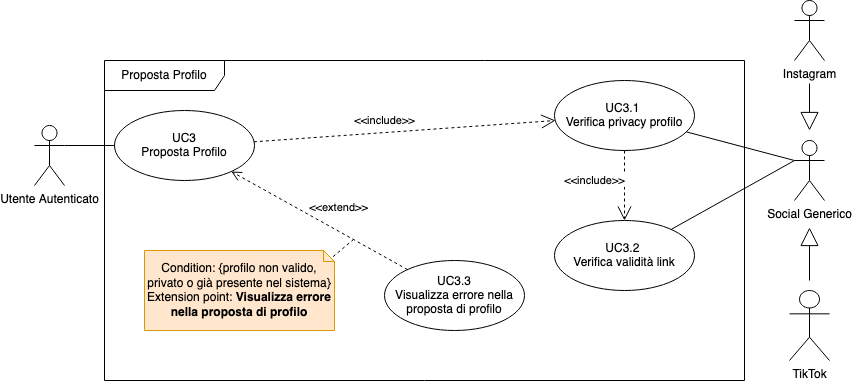
\includegraphics[scale=0.5]{UC_images/UC3.png}
\end{center}
\begin{itemize}
    \item \textbf{Attore primario}: Utente autenticato.
    \item \textbf{Precondizione}: Il sistema possiede una lista di profili social da cui effettuare il crawling dei dati.
    \item \textbf{Postcondizione}: Alla lista di profili da cui effettuare il crawling viene aggiunto il profilo indicato dall’utente e tutti i profili pubblici presenti nella lista amici del profilo suggerito.
    \item \textbf{Scenario principale}: 
    \begin{enumerate}
        \item L'utente autenticato accede al sistema;
        \item L’utente seleziona la funzionalità suggerisci un profilo;
        \item L’utente inserisce il link valido ad un profilo instagram o tiktok pubblico.
    \end{enumerate}
    \item \textbf{Estensioni}:
    \begin{itemize}
        \item Nel caso in cui l’utente inserisce un link non valido:
        \begin{enumerate}
            \item Il link non viene inserito nella lista;
            \item Viene visualizzato un messaggio di errore nella proposta di profilo (UC3.3 §);
            \item Viene fornita all’utente la possibilità di modificare il link.
        \end{enumerate}
        \item Nel caso in cui l’utente inserisce il link ad un profilo privato:
        \begin{enumerate}
            \item Il link non viene inserito nella lista;
            \item Viene visualizzato un messaggio di errore nella proposta di profilo (UC3.3 §).
        \end{enumerate}
        \item Nel caso in cui viene inserito un link valido ad un profilo pubblico già presente nel sistema:
        \begin{enumerate}
            \item Il link non viene inserito nella lista.
        \end{enumerate} 
    \end{itemize}
    \item Inclusioni:
    \begin{enumerate}
        \item Verifica privacy profilo (UC3.1).
    \end{enumerate}
\end{itemize}

\subsection{UC3.1 – Verifica privacy profilo}
\begin{itemize}
    \item \textbf{Attore primario}: Utente autenticato.
    \item \textbf{Attore secondario}: Social generico.
    \item \textbf{Precondizione}: L’utente ha richiesto l’aggiunta di un profilo social fornendone il link.
    \item \textbf{Postcondizione}: Il sistema sa se il profilo suggerito è pubblico o privato.

    \item \textbf{Scenario principale}: 
    \begin{enumerate}
        \item Il sistema chiede al social in questione se il profilo proposto è pubblico o privato;
        \item Il social in questione invia una risposta dicendo se il profilo è pubblico o privato.
    \end{enumerate}

    \item \textbf{Inclusioni}:
    \begin{enumerate}
        \item Verifica validità link (UC3.2 §).
    \end{enumerate}
\end{itemize}

\subsection{UC3.2 – Verifica validità link}
\begin{itemize}
    \item \textbf{Attore primario}: Utente autenticato.
    \item \textbf{Attore secondario}: Social generico.
    \item \textbf{Precondizione}: L’utente ha richiesto l’aggiunta di un profilo social fornendone il link.
    \item \textbf{Postcondizione}: Il sistema sa se il link fornito è valido.

    \item \textbf{Scenario principale}: 
    \begin{enumerate}
        \item Il sistema chiede al social in questione se il link è valido;
        \item Il social in questione invia una risposta dicendo se il link è valido o meno.
    \end{enumerate}
\end{itemize}

\subsection{UC3.3 – Visualizza errore nella proposta di profilo}
\begin{itemize}
    \item \textbf{Attore primario}: Utente autenticato.
    \item \textbf{Precondizione}: L’utente ha richiesto l’aggiunta di un profilo social fornendone un link non valido o di un profilo privato.
    \item \textbf{Postcondizione}: Viene visualizzato un messaggio di errore e il link non viene aggiunto al sistema.
    \item \textbf{Scenario principale}: 
    \begin{enumerate}
        \item L'inserimento del link nella lista fallisce;
        \item Viene visualizzato a schermo un messaggio di errore.
    \end{enumerate}
\end{itemize}
%\clearpage 
	\subsection{UC4 – Gestione Risultati}
\begin{center}
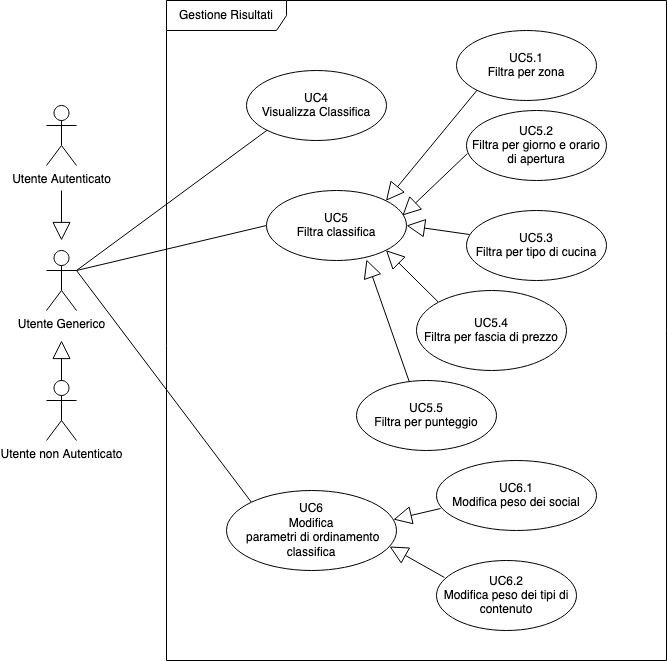
\includegraphics[scale=0.5]{UC_images/UC4.png}
\end{center}
\subsubsection{UC4.1 – Visualizza Classifica}
\begin{center}
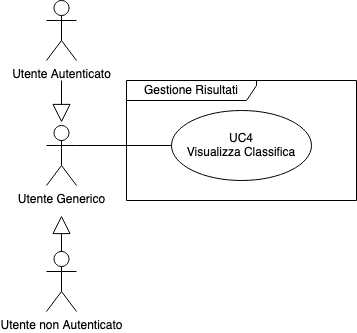
\includegraphics[scale=0.5]{UC_images/UC4-2.png}
\end{center}
\begin{itemize}
    \item \textbf{Attore primario}: Utente autenticato.
    \item \textbf{Precondizione}: L’utente si trova all’interno della piattaforma Sweeat.
    \item \textbf{Postcondizione}: L’utente visualizza a schermo la classifica dei migliori locali gastronomici prodotta dal sistema senza alcun filtro applicato e con i parametri di ordinamento di default.
    \item \textbf{Scenario principale}: 
    \begin{enumerate}
        \item Un utente generico accede al sistema;
        \item L’utente seleziona la funzionalità visualizza classifica.
    \end{enumerate}
\end{itemize}


	\subsection{UC5 – Filtra classifica}
\begin{center}
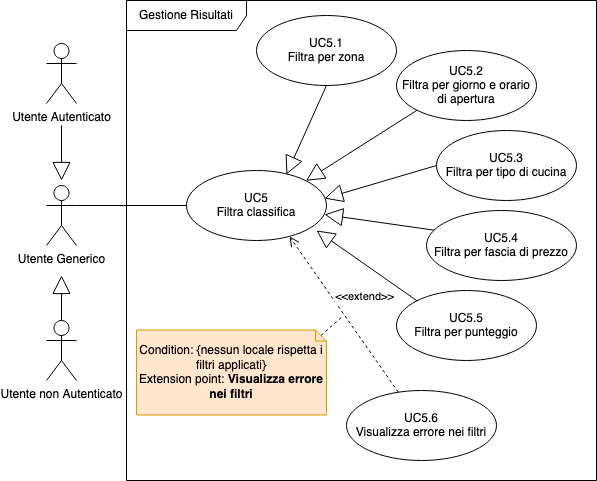
\includegraphics[scale=0.5]{UC_images/UC5.png}
\end{center}
\begin{itemize}
    \item \textbf{Attore primario}: Utente generico.
    \item \textbf{Precondizione}: L’utente sta visualizzando la classifica (UC3 §).
    \item \textbf{Postcondizione}: L’utente visualizza a schermo la classifica dei migliori locali gastronomici che rientrano all’interno dei filtri inseriti.
    \item \textbf{Scenario principale}: 
    \begin{enumerate}
        \item L’utente clicca il pulsante “Filtra Classifica”;
        \item L’utente applica dei filtri;
        \item L’utente clicca il pulsante “Applica Filtri”.
    \end{enumerate}

    \item \textbf{Generalizzazioni}:
    \begin{enumerate}
        \item Filtra per zona (UC5.1 §);
        \item Filtra per giorno e orario di apertura (UC5.2 §);
        \item Filtra per tipo di cucina (UC5.3 §);
        \item Filtra per fascia di prezzo (UC5.4 §);
        \item Filtra per punteggio (UC5.5 §).
    \end{enumerate}

    \item \textbf{Estensioni}:
    \begin{itemize}
        \item Nel caso in cui non ci sia nemmeno un locale che rispetta i filtri applicati:
        \begin{enumerate}
            \item Viene visualizzato un messaggio che informa l’utente del fatto che nessun locale rientra nei filtri inseriti (UC5.6 §);
            \item Viene fornita la possibilità di modificare i filtri.
        \end{enumerate}
    \end{itemize}
\end{itemize}

\subsubsection{UC5.1 – Filtra per zona}
\begin{itemize}
    \item \textbf{Attore primario}: Utente generico.
    \item \textbf{Precondizione}: L’utente sta visualizzando la classifica (UC4 §) e ha premuto il pulsante “Filtra Classifica”.
    \item \textbf{Postcondizione}: Il filtro in questione viene applicato.
    \item \textbf{Scenario principale}: 
    \begin{enumerate}
        \item L’utente digita il nome di uno o più luoghi;
        \item L’utente preme il pulsante invio.
    \end{enumerate}
\end{itemize}

\subsubsection{UC5.2 – Filtra per giorno e orario di apertura}
\begin{itemize}
    \item \textbf{Attore primario}: Utente generico.
    \item \textbf{Precondizione}: L’utente sta visualizzando la classifica (UC4 §) e ha premuto il pulsante “filtra classifica”.
    \item \textbf{Postcondizione}: Il filtro in questione viene applicato.
    \item \textbf{Scenario principale}: 
    \begin{enumerate}
        \item L’utente seleziona uno o più giorni della settimana da un checkbox;
        \item L’utente inserisce uno o più orari;
        \item L’utente clicca il pulsante “OK”.
    \end{enumerate}
\end{itemize}

\subsubsection{UC5.3 – Filtra per tipo di cucina}
\begin{itemize}
    \item \textbf{Attore primario}: Utente generico.
    \item \textbf{Precondizione}: L’utente sta visualizzando la classifica (UC4 §) e ha premuto il pulsante “Filtra Classifica”.
    \item \textbf{Postcondizione}: Il filtro in questione viene applicato.
    \item \textbf{Scenario principale}: 
    \begin{enumerate}
        \item L’utente seleziona uno o più tipi di cucina tra quelli proposti tramite un checkbox;
        \item L’utente clicca il pulsante “OK”.
    \end{enumerate}
\end{itemize}

\subsubsection{UC5.4 – Filtra per fascia di prezzo}
\begin{itemize}
    \item \textbf{Attore primario}: Utente generico.
    \item \textbf{Precondizione}: L’utente sta visualizzando la classifica (UC4 §) e ha premuto il pulsante “Filtra Classifica”.
    \item \textbf{Postcondizione}: Il filtro in questione viene applicato.
    \item \textbf{Scenario principale}: 
    \begin{enumerate}
        \item L’utente inserisce il valore minimo della fascia di prezzo;
        \item L’utente inserisce il valore massimo della fascia di prezzo;
        \item L’utente clicca il pulsante “OK”.
    \end{enumerate}
\end{itemize}

\subsubsection{UC5.5 – Filtra per punteggio}
\begin{itemize}
    \item \textbf{Attore primario}: Utente generico.
    \item \textbf{Precondizione}: L’utente sta visualizzando la classifica (UC4 §) e ha premuto il pulsante “filtra classifica”.
    \item \textbf{Postcondizione}: Il filtro in questione viene applicato.
    \item \textbf{Scenario principale}: 
    \begin{enumerate}
        \item L’utente inserisce il punteggio minimo;
        \item L’utente inserisce il punteggio massimo;
        \item L’utente clicca il pulsante “OK”.
    \end{enumerate}
\end{itemize}

\subsubsection{UC5.6 – Visualizza errore nei filtri}
\begin{itemize}
    \item \textbf{Attore primario}: Utente generico.
    \item \textbf{Precondizione}: L'utente ha inserito filtri ai quali non corrisponde alcun locale presente nel sistema.
    \item \textbf{Postcondizione}: Viene visualizzato un messaggio di errore.
    \item \textbf{Scenario principale}: 
    \begin{enumerate}
        \item L'utente inserisce dei filtri alla classifica;
        \item Nessun locale rientra nei filtri inseriti;
        \item Viene visualizzato a schermo un messaggio che informa l'utente di ciò che è accaduto.
    \end{enumerate}
\end{itemize}
%\clearpage 
	\subsection{UC6 – Modifica parametri di ordinamento classifica}
\begin{center}
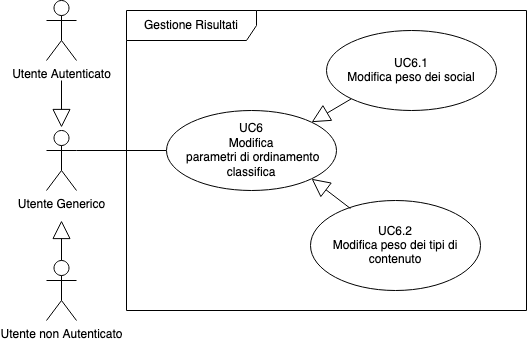
\includegraphics[scale=0.5]{UC_images/UC6.png}
\end{center}
\begin{itemize}
    \item \textbf{Attore primario}: Utente generico.
    \item \textbf{Precondizione}: L’utente sta visualizzando la classifica (UC3 §).
    \item \textbf{Postcondizione}: L’utente visualizza a schermo la classifica dei migliori locali gastronomici riordinata in base ai parametri di ordinamento inseriti.
    \item \textbf{Scenario principale}: 
    \begin{enumerate}
        \item L’utente clicca il pulsante “modifica parametri di ordinamento”;
        \item L’utente modifica i parametri di ordinamento;
        \item L’utente cicca il pulsante “applica parametri”.
    \end{enumerate}

    \item \textbf{Generalizzazioni}:
    \begin{enumerate}
        \item Modifica peso dei social (UC6.1 §);
        \item Modifica peso dei tipi di contenuto (UC6.2 §).
    \end{enumerate}

\end{itemize}

\subsubsection{UC6.1 – Modifica peso dei social }
\begin{itemize}
    \item \textbf{Attore primario}: Utente generico.
    \item \textbf{Precondizione}: L’utente sta visualizzando la classifica (UC §) e ha premuto il pulsante “Modifica Parametri di Ordinamento”.
    \item \textbf{Postcondizione}: Il parametro in questione viene applicato.
    \item \textbf{Scenario principale}: 
    \begin{enumerate}
        \item L’utente modifica il peso in percentuale che forniscono i contenuti di ciascun social tramite una barra percentuale;
        \item L’utente clicca il pulsante “OK”.
    \end{enumerate}
\end{itemize}

\subsubsection{UC6.2 – Modifica peso dei tipi di contenuto}
\begin{itemize}
    \item \textbf{Attore primario}: Utente generico.
    \item \textbf{Precondizione}: L’utente sta visualizzando la classifica (UC §) e ha premuto il pulsante “modifica parametri di ordinamento”.
    \item \textbf{Postcondizione}: Il parametro in questione viene applicato.
    \item \textbf{Scenario principale}: 
    \begin{enumerate}
        \item L’utente modifica il peso in percentuale che forniscono i tipi di contenuto (foto, post, stories, commenti) tramite una barra percentuale;
        \item L’utente clicca il pulsante “OK”.
    \end{enumerate}
\end{itemize}
	\subsection{UC7 – Ricerca di un locale tramite nome}
\begin{center}
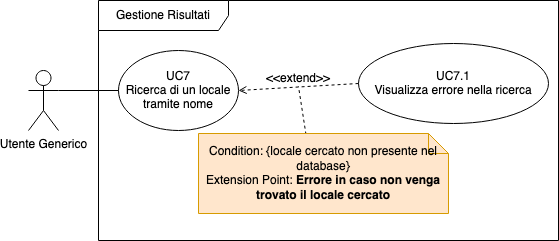
\includegraphics[scale=0.5]{UC_images/UC7.png} 
\end{center}
\begin{itemize}
    \item \textbf{Attore primario}: Utente generico.
    \item \textbf{Precondizione}: L'utente si trova all’interno della piattaforma Sweeat.
    \item \textbf{Postcondizione}: Viene visualizzato la lista dei locali ricercati.
    \item \textbf{Scenario principale}: 
    \begin{enumerate}
        \item L’utente va nella barra di ricerca della piattaforma;
        \item L’utente digita il nome del locale da cercare;
        \item L’utente clicca sul bottone di ricerca;
    \end{enumerate}
    \item \textbf{Estensioni}:
    \begin{itemize}
        \item Nel caso in cui l’utente l’utente inserisce il nome di un locale inesistente
	\begin{enumerate}  
		\item L’utente va nella barra di ricerca della piattaforma;
        \item L’utente digita il nome del locale da cercare;
        \item L’utente clicca sul bottone di ricerca; 
        \item Viene mostrato un messaggio d'errore, nel caso non sia presente alcun locale (UC7.1 §).
    	%Visualizzazione di un messaggio informando che non è presente nessun locale con tale nome e viene suggerita una lista di locali simili a quello ricercato.   
    \end{enumerate}
    \end{itemize}    
\end{itemize}

\subsubsection{UC7.1 – Visualizza errore nella ricerca}
\begin{itemize}
\item \textbf{Attore primario}: Utente Generico.
\item \textbf{Precondizione}: L'utente si trova all’interno della piattaforma Sweeat.
\item \textbf{Postcondizione}: Viene mostrato un messaggio d'errore e l'utente non è in grado di visualizzare il locale cercato.

\item \textbf{Scenario principale}:
\begin{enumerate}
	\item L'operazione di ricerca del locale desiderato fallisce;
	\item Viene mostrato il corrispondente messaggio d'errore;
	\item All'utente viene data la possibilità di visualizzare dei locali alternativi di cercare nuovamente il locale desiderato.
\end{enumerate}
\end{itemize}
	\subsection{UC8 – Visualizza informazioni locale}
\begin{center}
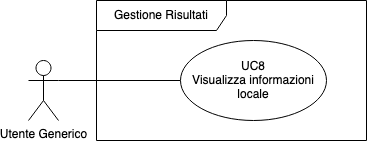
\includegraphics[scale=0.5]{UC_images/UC8.png} 
\end{center}
\begin{itemize}
    \item \textbf{Attore primario}: Utente Generico;
    \item \textbf{Precondizione}: L'utente ha svolto la funzione di ricerca di un locale o sta visualizzando la classifica;
    \item \textbf{Postcondizione}: Vengono visualizzate le informazioni di un locale.
    
    \item \textbf{Scenario principale}: 
    \begin{enumerate}
    \item L'utente seleziona un locale tra quelli presenti nella lista;
    \item Il sistema mostrerà all'utente le informazioni relative al locale scelto.
    \end{enumerate}
\end{itemize}

	\subsection{UC9 – Gestione lista dei locali preferiti}
\begin{center}
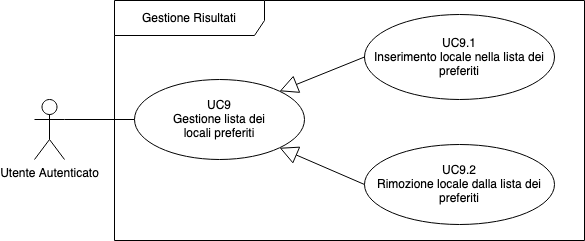
\includegraphics[scale=0.5]{UC_images/UC9.png} 
\end{center}
\begin{itemize}
    \item \textbf{Attore primario}: Utente autenticato.
    \item \textbf{Precondizione}: L'utente è autenticato e si trova all’interno della piattaforma Sweeat.
    \item \textbf{Postcondizione}: Viene visualizzata o modificata la lista dei locali preferiti.
    \item \textbf{Scenario principale}: L’utente accede alla funzionalità di gestione della lista dei locali preferiti cliccando su “Preferiti”.
    \item \textbf{Generalizzazioni}:
     \begin{enumerate}
        \item Inserimento di un locale nella lista dei locali preferiti (UC9.1 §).
        \item Rimozione di un locale dalla lista dei locali preferiti (UC9.2 §).
    \end{enumerate}
\end{itemize}
\subsubsection{UC9.1 – Inserimento locale nella lista dei preferiti}
\begin{itemize}
    \item \textbf{Attore primario}: Utente autenticato.
    \item \textbf{Precondizione}: L'utente è autenticato e si trova all’interno della piattaforma Sweeat.
    \item \textbf{Postcondizione}: Viene inserito il locale scelto dall’utente nella lista dei locali preferiti.
    \item \textbf{Scenario principale}: L’utente seleziona dalla lista dei locali il locale da inserire nella lista dei locali preferiti, cliccando su “Aggiungi ai Preferiti”.
\end{itemize}

\subsubsection{UC9.2 – Rimozione locale dalla lista dei preferiti}

\begin{itemize}
    \item \textbf{Attore primario}: Utente autenticato.
    \item \textbf{Precondizione}:  L’utente è autenticato nel sistema e c'è almeno un locale inserito nella lista dei locali preferiti dall’utente.
    \item \textbf{Postcondizione}: Viene rimosso il locale scelto dall’utente dalla lista dei locali preferiti.
    \item \textbf{Scenario principale}:
    \begin{enumerate}
        \item L’utente seleziona dalla lista dei locali preferiti il locale da rimuovere dalla lista dei locali preferiti;
        \item L’utente rimuove il locale da rimuovere dalla lista dei locali preferiti, cliccando su “Rimuovi dai Preferiti”.
    \end{enumerate}
\end{itemize}
	
	
	\pagebreak	
	\section{Requisiti}

\subsection{Introduzione}
In base a quanto definito nel documento \textit{\NdP}, nella sezione §2.2.3.4, il team DreamTeam ha classificato ed assegnato i requisiti come espresso nelle prossime righe.


	\subsection{Requisiti Funzionali}

\definecolor{darkblue}{cmyk}{99, 99, 0, 71}

\renewcommand{\arraystretch}{1.5}
\rowcolors{2}{gray!25}{white}
\begin{longtable}{ m{0.15\textwidth}<{\centering}  m{0.4\textwidth}<{\centering}  m{0.16\textwidth}<{\centering}  m{0.19\textwidth}<{\centering}}
	\rowcolor{darkblue}
	\textcolor{white}{\textbf{Requisito}} &\textcolor{white}{\textbf{Descrizione}}& \textcolor{white}{\textbf{Classificazione}} & \textcolor{white}{\textbf{Fonti}}\\ 

	R1FW1 & L’utente deve riuscire ad inserire i propri dati personali (nome, cognome, indirizzo e-mail e password) per effettuare la registrazione & \Ob & UCW1 \\	
	 
	R1FW2 & L’utente deve riuscire ad inserire i propri dati (indirizzo e-mail e password) per effettuare il login & \Ob & UCW2\\	

	R1FW3 & L’utente deve riuscire a recuperare la password, nel caso l’avesse dimenticata & \De & UCW3\\	
	 
	R1FE1 & All’utente viene mostrato un errore nel caso non inserisca correttamente il nome in fase di registrazione & \Ob & UCE1\\	
	 
 	R1FE2 & All’utente viene mostrato un errore nel caso non inserisca correttamente il cognome in fase di registrazione & \Ob & UCE2\\	
	 
	R1FE3 & All’utente viene mostrato un errore nel caso non inserisca correttamente l’indirizzo e-mail in fase di registrazione & \Ob & UCE3\\	

	R1FE4 & All’utente viene mostrato un errore nel caso non inserisca una password corretta in fase di registrazione & \Ob & UCE4\\	
	
	R1FE5 & All'utente viene mostrato un errore nel caso non inserisca correttamente l'indirizzo e-mail al login & \Ob & UCE5 \\
	 
	R1FE6 & All'utente viene mostrato un errore nel caso non inserisca correttamente la password al login & \Ob & UCE6 \\	 
	 
	R1FE7 & All’utente viene mostrato un errore nel caso non inserisca correttamente l’indirizzo e-mail nel recupero password & \Ob & UCE7\\	

	R1FW4 &	Un utente autenticato può accedere alla sua Area Personale & \Ob & UCW4 \\ 
	 
	R2FW4.1 & L’utente autenticato può collegare il proprio profilo Instagram  & \Ob & UCW4.1\\	
	 
	R2FE8 & All’utente autenticato viene mostrato un messaggio d’errore nel caso il collegamento al profilo Instagram non vada a buon fine & \Ob & UCE8\\	
	 
	R2FW4.2 & L’utente autenticato può collegare al proprio profilo l’account TikTok & \Ob & UCW4.2\\		 

	R2FE9 & All’utente autenticato viene mostrato un messaggio d’errore nel caso il collegamento al profilo TikTok non vada a buon fine  & \Ob & UCE9 \\		
	 
	R3FW4.3 & L’utente autenticato può modificare la password con cui accede al sistema & \Fa & UCW4.3\\				
	 
	R3FE15 & All’utente autenticato viene mostrato un errore nel caso non inserisca una password valida, in fase di modifica  & \Fa & UCE15\\			
	  	 	 	
	R1FW5 & L’utente autenticato può suggerire dei profili social da cui fare il crawling dei dati & \Ob & UCW5, UCW6\\		
	 
	R2FE10 & All’utente autenticato viene mostrato un messaggio d’errore nel caso suggerisca un profilo social inesistente & \De & UCE10\\		

	R2FE11 & All’utente autenticato viene mostrato un messaggio d’errore nel caso l’utente suggerito abbia un profilo privato & \De & UCE11\\
	 
	R2FE12 & All’utente autenticato viene mostrato un messaggio d’errore nel caso suggerisca un profilo già presente a sistema & \De & UCE12\\			
	 
	R1FW7 & L’utente può visualizzare la classifica con i locali presenti nel database della piattaforma & \Ob & UCW7\\	
	 
	R1FW8 & L’utente può filtrare la classifica & \Ob & UCW8\\		
	
	R2FE13 & Nel caso non ci sia alcun risultato compatibile con i filtri applicati, viene mostrato un errore & \De & UCE13\\	
	 
	R1FW8.1 & L’utente può filtrare la classifica dei locali presenti nel database del sistema in base alla zona & \Ob & UCW8.1\\	
	 
	R2FW8.2 & L’utente può filtrare la classifica dei locali presenti nel database del sistema per giorno ed orario di apertura & \De & UCW8.2\\	
	 
	R2FW8.3 & L’utente può filtrare la classifica dei locali presenti nel database del sistema in base al tipo di cucina & \De & UCW8.3\\	
	 
	R2FW8.4 & L’utente può filtrare la classifica dei locali presenti nel database del sistema per fascia di prezzo & \De & UCW8.4\\	 
	 
	R1FW8.5 & L’utente può filtrare la classifica dei locali presenti nel database del sistema in base al punteggio & \Ob & UCW8.5\\	 
	 
	R3FW9 & L’utente può modificare l’ordinamento di visualizzazione della classifica & \Fa & UCW9\\	
	 
	R3FW9.1 & L’utente può modificare la visualizzazione dei risultati della classifica, impostando il peso dei social & \Fa & UCW9.1\\	 
	 
	R3FW9.2 & L’utente può modificare la visualizzazione dei risultati della classifica, impostando il peso dei tipi di contenuto & \Fa & UCW9.2\\	  
	 
	R1FW10 & L’utente può cercare un locale presente nel database del sistema tramite il suo nome & \Ob & UCW10 \\	 
	 
	R2FE14 & All’utente viene mostrato un errore in caso il locale cercato non sia presente nel sistema & \De & UCE14\\	 
	 	 
	R1FW11 & L’utente può visualizzare le informazioni di un locale presente nel sistema & \Ob & UCW11\\	 	 	 	

	R2FW12 & L’utente può aggiungere un locale alla lista dei preferiti & \De &  UCW12\\

	R2FW13 & L’utente può rimuovere un locale dalla lista dei preferiti & \De & UCW13\\

	R3F1 & L’utente può suggerire delle modifiche da apportare relative alle informazioni di un locale & \Fa & \Di \\

	\hiderowcolors \caption{Requisiti Funzionali}
\end{longtable}

\clearpage
	\subsection{Requisiti di Qualità}

\definecolor{darkblue}{cmyk}{99, 99, 0, 71}

\renewcommand{\arraystretch}{1.5}
\rowcolors{2}{gray!25}{white}
\begin{longtable}{ m{0.15\textwidth}<{\centering}  m{0.4\textwidth}<{\centering}  m{0.16\textwidth}<{\centering}  m{0.19\textwidth}<{\centering}}
	\rowcolor{darkblue}
	\textcolor{white}{\textbf{Requisito}} &\textcolor{white}{\textbf{Descrizione}}& \textcolor{white}{\textbf{Classificazione}} & \textcolor{white}{\textbf{Fonti}}\\ 

	R1Q1 & Il sistema dovrà essere sviluppato secondo quanto espresso nel documento \textit{\NdP} & \Ob & \Di \\
	
	R1Q2 & Deve essere fornito un documento di sintesi in lingua italiana sui limiti dei social utilizzati & \Ob & \Ca \\
	
	R1Q3 & Deve essere fornita una documentazione dettagliata in lingua italiana di tutte le API\textsuperscript{G} & \Ob & \Ca \\

	R1Q4 & Deve essere fornito un documento in lingua italiana realtivo ai limiti di servizi e algoritmi usati per estrarre la valutazione di un luogo di interesse & \Ob & \Ca \\

	R1Q5 & Il codice sorgente della piattaforma sarà reperibile su \textit{GitHub} & \Ob & VerbaleInterno-2021.11.29 \\
	
	R1Q6 & Dovrà essere realizzato un manuale interno in lingua italiana  & \Ob & \Di \\

	\hiderowcolors \caption{Requisiti di Qualità}
\end{longtable}

\clearpage
	\subsection{Requisiti di Vincolo}

\definecolor{darkblue}{cmyk}{99, 99, 0, 71}

\renewcommand{\arraystretch}{1.5}
\rowcolors{2}{gray!25}{white}
\begin{longtable}{ m{0.15\textwidth}<{\centering}  m{0.4\textwidth}<{\centering}  m{0.16\textwidth}<{\centering}  m{0.19\textwidth}<{\centering}}
	\rowcolor{darkblue}
	\textcolor{white}{\textbf{Requisito}} &\textcolor{white}{\textbf{Descrizione}}& \textcolor{white}{\textbf{Classificazione}} & \textcolor{white}{\textbf{Fonti}}\\ 

	R1V1 & L’interfaccia utente del sistema dovrà essere sviluppato sfruttando il framework React & \Ob & \Vi{} 2022-01-13 \\	

	R1V2 & Il sistema dovrà funzionare sul browser Chrome dalla versione più recente (97.0.4692) & \Ob & \Ve{} 2022-01-26 \\	
	 
	R1V3 & Il sistema dovrà funzionare sul browser Microsoft Edge dalla versione più recente (96.0.1031.0) & \Ob & \Ve{} 2022-01-26 \\	

	R1V4 & Il sistema dovrà funzionare sul browser Firefox dalla versione più recente (96.0.2) & \Ob & \Ve{} 2022-01-26 \\	
	 
	R1V5 & Il sistema dovrà funzionare sul browser Safari dalla versione più recente (15.3) & \Ob & \Ve{} 2022-01-26 \\	
	 
	R1V6 & Il sistema dovrà sfruttare i servizi offerti da AWS\textsuperscript{G} & \Ob & \Ca \\	
	 
	R2V1 & Il sistema dovrà sfruttare il database Amazon Aurora Serverless\textsuperscript{G} & \De & \Vi{} 2022-01-13 \\
	
	R1V7 & Il sistema dovrà sfruttare il servizio di calcolo AWS Lambda\textsuperscript{G} & \Ob & \Ca \\	
	 
	R1V8 & Il sistema dovrà sfruttare il servizio AWS API Gateway\textsuperscript{G} & \Ob & \Ca \\
	
	R1V9 & Il sistema dovrà sfruttare il servizio Amazon Rekognition\textsuperscript{G} & \Ob & \Ca \\
		
	R1V10 & Il sistema dovrà sfruttare il servizio Amazon Comprehend\textsuperscript{G} & \Ob & \Ca \\	 

	R2V2 & Le API per lo sviluppo del crawler Instagram dovranno essere sviluppate in Python & \De & \Vi{} 2022-01-13 \\	
	 
	R2V3 & Le API per lo sviluppo del crawler TikTok dovranno essere sviluppate in Python & \De & \Vi{} 2022-01-13 \\	
	 
	R1V11 & È necessario sfruttare un’architettura a microservizi\textsuperscript{G}  & \Ob & \Ca \\	
	 
	R1V12 & È necessario non superare la soglia di 2000\$ di credito per i servizi offerti da AWS & \Ob & \Ve{} 2022-01-26 \\	
	
	\hiderowcolors \caption{Requisiti di Vincolo}
\end{longtable}

\pagebreak
	\subsection{Requisiti Prestazionali}

Non sono stati individuati requisiti prestazionali per quanto riguarda i requisiti obbligatori. I servizi di AWS utilizzati per realizzare la piattaforma non presentano problemi a livello di performance. 	
	\subsection{Tracciamento}

\subsubsection{Fonte - Requisiti}

\definecolor{darkblue}{cmyk}{99, 99, 0, 71}

\begin{table}[!htbp]
\rowcolors{2}{gray!25}{white}
\renewcommand{\arraystretch}{1.5}
\begin{tabular}{ m{0.3\textwidth}<{\centering}  m{0.65\textwidth}<{\centering} }
	\rowcolor{darkblue}
	\textcolor{white}{\textbf{Fonte}} &\textcolor{white}{\textbf{Requisiti}}\\ 

	Capitolato & R1Q2, R1Q3, R1Q4, R1V6, R1V7, R1V8, R1V9, R1V10, R1V11\\	

	Decisione Interna & R3F1, R1Q1, R1Q6 \\
	
	\Vi{} 2022-01-13 & R1V1, R2V1, R2V2, R2V3 \\
	
	\Vi{} 2021-11-29 & R1Q5 \\
	
	\Ve{} 2022-01-26 & R1V2, R1V3, R1V4, R1V5, R1V12 \\

\end{tabular}
\caption{Tabella di tracciamento Fonte - Requisiti (1)}
\end{table}

\pagebreak
\subsubsection{Fonte - Requisiti}

\begin{table}[!htbp]
\rowcolors{2}{gray!25}{white}
\renewcommand{\arraystretch}{1.5}
\begin{tabular}{ m{0.15\textwidth}<{\centering}  m{0.3\textwidth}<{\centering} }
	\rowcolor{darkblue}
	\textcolor{white}{\textbf{Fonte}} &\textcolor{white}{\textbf{Requisiti}}\\ 

	UCW1 & R1FW1\\	
	 
	UCW2 & R1FW2\\	

	UCW3 & R1FW3\\	
	 
	UCE1 & R1FE1\\	
	 
	UCE2 & R1FE2\\	
	 
	UCE3 & R1FE3\\	

	UCE4 & R1FE4\\	
	
	UCE5 & R1FE5\\
	 
	UCE6 & R1FE6\\	 
	 
	UCE7 & R1FE7\\	

	UCW4 & R1FW4\\ 
	 
	UCW4.1 & R1FW4.1\\	
	 
	UCE8 & R1FE8 \\	
	 
	UCW4.2 & R1FW4.2\\		 

	UCE9 & R1FE9\\		
	 
	UCW4.3 & R3FW4.3 \\				
	 
	UCE15 & R3FE15\\			
	  	 	 	
	UCW5 & R1FW5\\		
	 
	UCW6 & R1FW5 \\
	
	UCE10 & R2FE10 \\

\end{tabular}
\begin{tabular}{ m{0.15\textwidth}<{\centering}  m{0.3\textwidth}<{\centering} }
	\rowcolor{darkblue}
	\textcolor{white}{\textbf{Fonte}} &\textcolor{white}{\textbf{Requisiti}}\\ 

	UCE11 & R2FE11\\
	 
	UCE12 & R2FE12 \\			
	 
	UCW7 & R1FW7 \\	
	 
	UCW8 & R1FW8 \\		
	
	UCE13 & R2FE13  \\	
	 
	UCW8.1 & R1FW8.1 \\	
	 
	UCW8.2 & R2FW8.2 \\	
	 
	UCW8.3 & R2FW8.3\\	
	 
	UCW8.4 & R2FW8.4 \\	 
	 
	UCW8.5 & R1FW8.5 \\	 
	 
	UCW9 & R3FW9 \\	
	 
	UCW9.1 & R3FW9.1\\	 
	 
	UCW9.2 & R3FW9.2\\	  
	 
	UCW10 & R1FW10 \\	 
	 
	UCE14 & R2FE14\\	 
	 	 
	UCW11 & R1FW11\\	 	 	 	

	UCW12 & R2FW12\\

	UCW13 & R2FW13 \\

	R1FW1 & UCW1 \\

\end{tabular}
\caption{Tabella di tracciamento Fonte - Requisiti (2)}
\end{table}

\pagebreak

\subsubsection{Requisito - Fonti}

\begin{table}[!htbp]
\rowcolors{2}{gray!25}{white}
\renewcommand{\arraystretch}{1.5}
\begin{tabular}{ m{0.125\textwidth}<{\centering}  m{0.15\textwidth}<{\centering} }
	\rowcolor{darkblue}
	\textcolor{white}{\textbf{Requisito}} &\textcolor{white}{\textbf{Fonti}}\\ 	
	 
	R1FW2 & UCW2\\	

	R1FW3 & UCW3\\	
	 
	R1FE1 & UCE1\\	
	 
 	R1FE2 & UCE2\\	
	 
	R1FE3 & UCE3\\	

	R1FE4 & UCE4\\	
	
	R1FE5 & UCE5 \\
	 
	R1FE6 & UCE6 \\	 
	 
	R1FE7 & UCE7\\	

	R1FW4 & UCW4 \\ 
	 
	R1FW4.1 & UCW4.1\\	
	 
	R1FE8 & UCE8\\	
	 
	R1FW4.2 & UCW4.2\\		 

	R1FE9 & UCE9 \\		
	 
	R3FW4.3 & UCW4.3\\				
	 
	R3FE15 & UCE15\\			
	  	 	 	
	R1FW5 & UCW5, UCW6\\		
	 
	R2FE10 & UCE10\\
	
	R2FE11 & UCE11\\
	 
	R2FE12 & UCE12\\	
	
	R1FW7 & UCW7\\

\end{tabular}
\begin{tabular}{ m{0.125\textwidth}<{\centering}  m{0.15\textwidth}<{\centering} }
	\rowcolor{darkblue}
	\textcolor{white}{\textbf{Requisito}} &\textcolor{white}{\textbf{Fonti}}\\ 			 
	 
	R1FW8 & UCW8\\		
	
	R2FE13 & UCE13\\	
	 
	R1FW8.1 & UCW8.1\\	
	 
	R2FW8.2 & UCW8.2\\	
	 
	R2FW8.3 & UCW8.3\\	
	 
	R2FW8.4 & UCW8.4\\	 
	 
	R1FW8.5 & UCW8.5\\	 
	 
	R3FW9 & UCW9\\	
	 
	R3FW9.1 & UCW9.1\\	 
	 
	R3FW9.2 & UCW9.2\\	  
	 
	R1FW10 & UCW10 \\	 
	 
	R2FE14 & UCE14\\	 
	 	 
	R1FW11 & UCW11\\	 	 	 	

	R2FW12 & UCW12\\

	R2FW13 & UCW13\\

	R3F1 & \Di \\
	
	R1Q1 & \Di \\
	
	R1Q2 & \Ca \\
	
	R1Q3 & \Ca \\
	
	R1Q4 &  \Ca \\
	
	R1Q5 & \Vi{} 2021-11-29\\
	
\end{tabular}
\begin{tabular}{ m{0.125\textwidth}<{\centering}  m{0.15\textwidth}<{\centering} }
	\rowcolor{darkblue}
	\textcolor{white}{\textbf{Requisito}} &\textcolor{white}{\textbf{Fonti}}\\ 

	R1Q6 & \Di \\

	R1V1 & \Vi{} 2022-01-13 \\	

	R1V2 & \Ve{} 2022-01-26 \\	
	 
	R1V3 & \Ve{} 2022-01-26 \\	

	R1V4 & \Ve{} 2022-01-26 \\	
	 
	R1V5 & \Ve{} 2022-01-26 \\	
	 
	R1V6 & \Ca \\	
	 
	R2V1 & \Vi{} 2022-01-13 \\
	
	R1V7 & \Ca \\	
	 
	R1V8 & \Ca \\	 
	
	R1V9 & \Ca \\	
	
	R1V10 & \Ca \\
	
	R1V11 & \Ca \\

	R2V2 & \Vi{} 2022-01-13 \\	
	 
	R2V3 & \Vi{} 2022-01-13 \\	
	 
	R1V12 & \Ve{} 2022-01-26 \\	

\end{tabular}
\caption{Tabella di tracciamento Requisito - Fonti}
\end{table}

\subsubsection{Riepilogo Requisiti}

\begin{table}[!htbp]
\rowcolors{2}{gray!25}{white}
\renewcommand{\arraystretch}{1.5}
\begin{tabular}{ m{0.175\textwidth}<{\centering}  m{0.175\textwidth}<{\centering}  m{0.175\textwidth}<{\centering}  m{0.175\textwidth}<{\centering}  m{0.175\textwidth}<{\centering} }
	\rowcolor{darkblue}
	\textcolor{white}{\textbf{Tipologia}} &\textcolor{white}{\textbf{\Ob}}& \textcolor{white}{\textbf{\De}} & \textcolor{white}{\textbf{\Fa}}&\textcolor{white}{\textbf{Totale}}\\ 
	Funzionale & 21 & 11 & 6 & 38\\	
	Qualità & 6 & 0 & 0 & 6 \\	
	Vincolo & 12 & 3 & 0 & 15 \\	
	\textbf{Totale} & 39 & 	14 & 6 & 59
\end{tabular}
\caption{Riepilogo dei Requisiti}
\end{table}	
	
\end{document}
